% vim: set tw=78 tabstop=4 shiftwidth=4 aw ai:

\chapter{Improved Multimedia Distribution in Peer-to-Peer Networks}
\label{chapter:multimedia-dist}

A large part of content distribution in the Internet is currently video
content. Video content means large files, typically movie files of CD or DVD
size. File size increases if the bitrate or resolution increases.

Apart from movie files, sites such as YouTube, focusing on small videos that
are published by average users are attracting millions of users. Content is
accessed many times and transferred across the Internet.

A Peer-to-Peer protocol and BitTorrent, in particular, is one of the most
adequate solution for distributing large content. Rapid creation of swarms,
tit-for-tat, rarest-piece first allow BitTorrent to rapidly distributed files
among peers. When thinking about video content, this mode is known as offline
playback -- the video file is downloaded and subsequently rendered. Separate
approaches are to be undertaken for Video-on-Demand and Live Streaming as
described in Section~\ref{subsec:multimedia-dist:video-consumption-production}.

Video-on-Demand refers to rendering video content that is already stored (in
full size) on a given server or peer. Video-on-Demand content may be
fast-forwarded or rewound to the desired position. Sites such as YouTube or
Vimeo are providing VoD content. Live Streaming content is content that is
generated in real time; typically this also incurs significant constraints on
network latency as data has to be delivered as it is generated. Live Streaming
uses cameras and video devices that capture real activities and delivery them
to the network at the same time.

Video files are actually a set of frames (images) that are played back at a
given rate. Most of the time, this rate is 24 fps (frames per second) which is
enough to ``fool'' the human brain into thinking it happens in real time. A
movie file possesses multiple features that are detailed in
Section~\ref{subsec:multimedia-dist:video-keywords}: video rate, resolution, container, codec.

Recent years have seen the proliferation of HD content. HD -- High Definition
-- characterizes video files possessing a large resolution. Common HD video
resolution is 1280x720 pixels, also known as 720p, and 1920x1080 pixels, also
known as 1080p. HD videos use wide screen aspect ratio (16:9). HD videos own
their proliferation to ever increasing computing power (for decoding and
rendering video files), storage space (for storing actual files) and network
bandwidth (allowing transfer of information).

Sites such as YouTube and Vimeo are able to provide HD videos. HD refers
strictly to the resolution of the video file. It makes no assumption around
the codec technology of video bitrate; one may find an HD asset to be of lower
quality than that of SD (standard definition) video because of its poorer
codec or lower bitrate.

The proliferation of HD content has also meant the proliferation of HD-able
video formats (HDCAM, D5 HD, AVCHD) and video devices. Modern video cameras
are HD-able, the recent Blu-ray disc is typically using HD media, and TV sets
nowadays are capable of rendering HD content.

A specialized media device is the Set-top Box (STB). A set-top box connects to
a TV and an external source of signal and generated required content for the
TV set. Set-top boxes form a more generic device than that of a TV set, as a
set-top box may integrated multiple features on its firmware. For example, the
Pioneer NextShare STB that is used in the P2P-Next project integrates P2P
facilities, social networking, per-user customization, remote connections and
others.

\begin{figure}
  \centering
  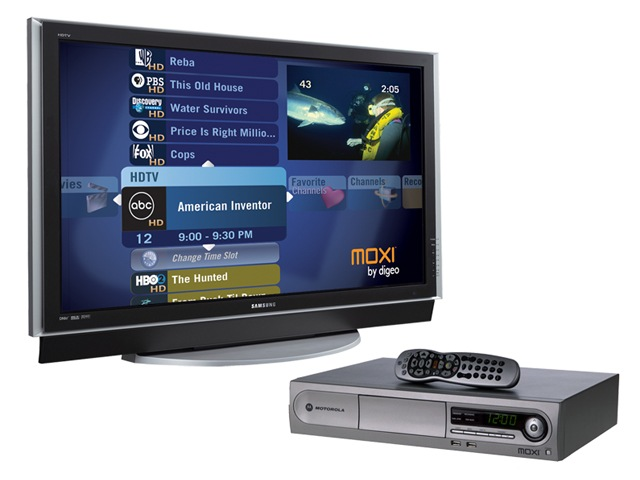
\includegraphics[width=0.5\textwidth]{src/img/multimedia-dist/stb}
  \caption{Set-top Box}
  \label{fig:multimedia-dist:stb}
\end{figure}

Set-top boxes are main components in IPTV networks as they may be easily
connected to an IP network and decode video streaming provided through the
network connection.

\section{Video Content Creation and Processing}
\label{sec:multimedia-dist:video}

Video content forms the most heavily used traffic class in the Internet. HTTP,
Peer-to-Peer, Flash and owe the greatest component of their bandwidth
consumption to video content\footnote{Sandvine: Global Broadband Trends,
\url{http://www.sandvine.com/news/global\_broadband\_trends.asp}}. With the ever
increasing bandwidth in the Internet video content demand is increasing
itself. Although poised by legal issues, Peer-to-Peer traffic is currently
made up of video content.

Video content is, at its base, a series of frames that are rendered in a fast
pace by a video player. Video files may be streamed, allowing the user to view
content without having access to the complete file. In order to reduce the
size of a video file, codecs are typically used. A codec will use lossy or
lossless data compression to diminish the size of a video file.

Video content/stream is provided together with audio stream inside a
container. An \textbf{An audio video container} file is used to identify and
interleave different multimedia data types. It usually stores different audio,
video and subtitle streams.

\subsection{Video Keywords}
\label{subsec:multimedia-dist:video-keywords}

\subsubsection{Audio Video Containers}

\textbf{Audio Video Interleave}, known by its acronym \textbf{AVI}, is the
most popular multimedia container used today, introduced by Microsoft in 1992.
An AVI file may carry audio/visual data in virtually any compression scheme,
including Full Frame (Uncompressed), Intel Real Time (Indeo), Cinepak, Motion
JPEG, MPEG, VDOWave, RealVideo and MPEG-4 Video.

The \textbf{.m2ts} or \textbf{.mts} is a filename extension used for the BDAV
MPEG-2 Transport Stream container file format. It is used for multiplexing
audio, video and other streams. It is based on the MPEG-2 transport stream
container. This container format is commonly used for high definition video on
Blu-ray Disc and AVCHD.

\textbf{Ogg} is a free, open standard container format maintained by the
Xiph.Org Foundation. The creators of the Ogg format state that it is
unrestricted by software patents and is designed to provide for efficient
streaming and manipulation of high quality digital multimedia. In the Ogg
multimedia framework, \textit{Theora} provides a lossy video layer. The audio
layer is most commonly provided by the music-oriented \textit{Vorbis} format
but other options include the human speech compression codec \textit{Speex},
the lossless audio compression codec \textit{FLAC}, and \textit{OggPCM}.

\textbf{MP4} is MPEG-4 Part 14, a multimedia container format standard,
specified as a part of MPEG-4 and should not be confused with MPEG-4.

\subsubsection{Audio}

The sound is a mechanical wave, an oscillation, represented in analog devices
as a signal. Any wave can be expressed as a sum of a (possibly infinite) set
of simple oscillating functions (sines and cosines), with a particular
frequency, amplitude and phase. Frequency is measured in Hz. The sound level,
which is related with the amplitude is measured in \textbf{decibels (dB)}, a
logarithmic unit.

To digitally represent sampled analog signals, \textbf{Pulse-code modulation
(PCM)} is used. The magnitude of the analogue signal is sampled regularly at
uniform intervals, with each sample being quantized to the nearest value
within a range of digital steps.

\textbf{Decibels relative to full scale}, commonly abbreviated \textbf{dBFS},
measures decibel amplitude levels in digital systems, relative to the maximum
available peak level, which is assigned to 0 dBFS. So as the sound gets more
silent, the dBFS values get smaller bellow zero. The complete silence is minus
infinite dBFS.

PCM streams have two basic properties that determine their fidelity to the
original analog signal:
\begin{itemize}
  \item \textbf{sampling rate (sampling frequency)}: the number of times per
  second that samples are taken;
  \item \textbf{bit depth}: the number of possible digital values that each
  sample can take.
\end{itemize}

The \textbf{Nyquist-Shannon sampling theorem} states that perfect
reconstruction of a signal is possible when the sampling frequency is greater
than twice the maximum frequency of the signal being sampled.

Typical sampling rates:
\begin{itemize}
  \item \textbf{8,000 Hz}: telephone transmissions;
  \item \textbf{22,050 Hz}: low quality sound, comparable with early 20th
  century audio formats like gramophone records;
  \item \textbf{44,100 Hz}: audio CD quality, originally chosen by Sony.
  \item \textbf{48,000 Hz}, \textbf{96,000 Hz} and \textbf{192,000 Hz}:
  professional digital audio, used for example in recording studios.
  DVD-Audio, BD-ROM audio tracks and HD-DVD audio tracks support them.
\end{itemize}

Typical bit depths:
\begin{itemize}
  \item \textbf{8-bit}: low quality sound, comparable with early 20th century
  audio formats like gramophone records;
  \item \textbf{16-bit}: audio CD quality, originally chosen by Sony.
  \item \textbf{24-bit}: professional digital audio, used for examples in
  recording studios. DVDs support this bit depth.
\end{itemize}

The audio stream is also characterized by the \textbf{number of channels},
which can be \textbf{mono}, with just one channel, \textbf{stereo}, with two
channels, or \textbf{surround}, with more channels. The surround
configurations are usually expressed with two numbers separated by a dot, like
2.1, 5.1, 5.0 etc.  The first one represents the number of channels with full
bandwidth and the second one with low frequency (bass).

\subsubsection{Video}

Electronic screens render colors using the \textbf{RGB color model}, which is
an additive color model in which red, green and blue light are added together
with various intensities to reproduce a broad array of colors.  Every pixel on
a screen contains three dots, one red, one green and one blue and their
intensity determines the hue. For example when all of them are at the lowest
intensity black is obtained and when all are at the highest intensity, the
pixel gets white.

The \textbf{frame rate} or \textbf{frame frequency} (\textbf{frames per
second} abbreviated as \textbf{fps}) is the number of still pictures per
second for video. Typical values for this characteristic are between 25 and 30
fps. Standards:
\begin{itemize}
  \item \textbf{PAL} (Europe, Asia, Australia etc.) and \textbf{SECAM}
  (France, Russia, parts of Africa etc.): 25 fps;
  \item \textbf{NTSC} (USA, Canada, Japan etc.): 29,97 fps;
  \item \textbf{Film} (cinematic motion picture): 24 fps.
\end{itemize}

Video can be interlaced or progressive. \textbf{Interlacing} was invented as a
way to achieve good visual quality within the limitations of a narrow
bandwidth. The horizontal scan lines of each interlaced frame are numbered
consecutively and partitioned into two fields: the odd field (upper field)
consisting of the odd-numbered lines and the even field (lower field)
consisting of the even-numbered lines. NTSC, PAL and SECAM are interlaced
formats. Abbreviated video resolution specifications often include an
\textit{i} to indicate interlacing. For example, PAL video format is often
specified as 576i50, where 576 indicates the vertical line resolution, i
indicates interlacing, and 50 indicates 50 fields (half-frames) per second.
\textbf{Progressive} or \textbf{noninterlaced scanning} is a method for
displaying, storing or transmitting moving images in which all the lines of
each frame are drawn in sequence.

The \textbf{display resolution} is the size of a video image, which is
measured in pixels for digital video, or horizontal scan lines and vertical
lines of resolution for analog video.

\textbf{Pixel aspect ratio} (often abbreviated \textbf{PAR}) is a mathematical
ratio that describes how the width of a pixel in a digital image compares to
the height of that pixel.

The \textbf{aspect ratio} or \textbf{display aspect ratio} (often abbreviated
\textbf{DAR}) of an image is the ratio of the width of the image to its
height, expressed as two numbers separated by a colon. Common aspect ratios
used:
\begin{itemize}
  \item \textbf{4:3}: standard definition;
  \item \textbf{16:9}: high definition (wide screen);
  \item \textbf{16:10 (8:5)}: wide screen computer monitors.
\end{itemize}

The number of distinct colors that can be represented by a pixel depends on
the number of \textbf{bits per pixel (bpp)}, also known as \textbf{color
depth}.

The video quality can be evaluated with a metric like \textbf{PSNR (Peak
signal-to-noise ratio)}, which is the ratio between the maximum possible power
of a signal and the power of corrupting noise that affects the fidelity of its
representation. It is usually expressed in dB.

\subsubsection{Television Systems}

\textbf{Standard-definition television (SDTV)} is a term usually used in
reference to digital television, in particular when broadcasting at the same
(or similar) resolution as analog systems. In the USA, SDTV refers to digital
television broadcast in 4:3 aspect ratio, the same aspect ratio as NTSC signal
known as 480i. In the UK and most of Europe standard-definition television is
mostly shown with a 16:9 aspect ratio as most people have a television with a
16:9 aspect ratio. The 16:9 aspect ratio is also known as 576i.

\textbf{High-definition television (HDTV or just HD)} refers to video having
resolution substantially higher than traditional television systems
(standard-definition TV, or SDTV, or SD). HD has one or two million pixels per
frame, roughly five times that of SD.

HDTV broadcast systems are identified with three major parameters:
\begin{itemize}
  \item \textbf{Frame size} in pixels is defined as number of horizontal
  pixels x number of vertical pixels, for example 1280 x 720 or 1920 x 1080.
  Often the number of horizontal pixels is implied from context and is
  omitted, as in the case of 720p and 1080p.
  \item \textbf{Scanning system} is identified with the letter \textit{p} for
  progressive scanning or \textit{i} for interlaced scanning.
  \item \textbf{Frame rate} is identified as number of video frames per
  second.
\end{itemize}

For example, 1920 x 1080p25 identifies progressive scanning format with 25
frames per second, each frame being 1,920 pixels wide and 1,080 pixels high.

The \textit{1080p}, with the resolution of 1920x1080 pixels is used by
\textbf{Full HD} and HD ready 1080p TV displays. The ratio of this resolution
is 16:9.

\subsection{Codecs}
\label{subsec:multimedia-dist:codecs}

\subsubsection{Multimedia Compression Standards}

A wide variety of methods are used to compress video streams. Video data
contains spatial and temporal redundancy, making uncompressed video streams
extremely inefficient. The most common modern standards are MPEG-2, used for
DVD and satellite television, and MPEG-4, used for home video. Both of these
standards are lossy data compressions, which lose the quality of the image in
order to gain smaller movies.

The \textit{.mpg} extension usually referes to one of a number of file
extensions for MPEG-1 or MPEG-2 audio and video compression.

\textbf{MPEG-4} is a collection of methods defining compression of audio and
visual (AV) digital data, in a set of standards developed in 1998 by ISO/IEC.
Every standard is termed "part". For example:
\begin{itemize}
  \item \textbf{Part 1} is titled \textbf{Systems}.
  \item \textbf{Part 2} is named \textbf{Visual} and includes \textit{Advanced
  Simple Profile}, used by codecs such as DivX, Xvid and Quicktime 6).
  \item \textbf{Part 3} is named \textbf{Audio} and is a set of compression
  codecs for perceptual coding of audio signals, including some variations of
  \textit{Advanced Audio Coding (AAC)} as well as other audio/speech coding
  formats and tools.
  \item \textbf{Part 10} is \textbf{Advanced Video Coding (AVC)}, which is a
  codec for video signals which is technically identical to the ITU-T
  \textit{H.262} standard.
  \item \textbf{Part 14} is named \textbf{MP4 file format}, which is the
  designed container file format for MPEG-4 content.
  \item \textbf{Part 15} for \textbf{Advanced Video Coding (AVC) file format},
  for storage of Part 10 video.
\end{itemize}

\paragraph{Audio Compression}

The most common lossless audio compression formats are \textbf{FLAC (Free
Lossless Audio Codec)}, which is open, and \textbf{Monkey's audio (APE)},
which is a proprietary format. Other audio lossless compression technologies
are \textbf{Apple Lossless}, \textbf{MPEG-4 ALS (Audio Lossless Coding)} etc.

\textbf{MP2} is an abbreviation from MPEG-1 Audio Layer II and should not be
confused with MPEG-2.

\textbf{MPEG-1} or \textbf{MPEG-2 Audio Layer 3 (or III)}, more commonly
referred to as \textbf{MP3}, is a patented digital audio encoding format using
a form of lossy data compression. It is a common audio format for consumer
audio storage, as well as a de facto standard of digital audio compression for
the transfer and playback of music on digital audio players.

\textbf{Vorbis} is a free software / open source project headed by the
Xiph.Org Foundation (formerly Xiphophorus company). The project produces an
audio format specification and software implementation (codec) for lossy audio
compression. Vorbis is most commonly used in conjunction with the Ogg
container format and it is therefore often referred to as \textbf{Ogg Vorbis}.

\paragraph{Video Compression}

\textbf{MPEG-4 Part 2 (Visual)} includes codecs such as DivX, Xvid, Quicktime
6 Nero Digital.  It is compatible with H.263.

\textbf{H.264/MPEG-4 Part 10} or \textbf{AVC (Advanced Video Coding)} is a
more performant video compression standard from MPEG-4.

\textbf{Theora} is a free lossy video compression format.[5] It is developed
by the Xiph.Org Foundation and distributed without licensing fees alongside
their other free and open media projects, including the Vorbis audio format
and the Ogg container.

\textbf{VP8} is an open video compression format released by Google,
originally created by On2 Technologies.

\subsection{Video Consumption and Production}
\label{subsec:multimedia-dist:video-consumption-production}

Video content is tipically streamed from a video source (server) to a series
of video consumers. Classical television uses air or cable as support for
delivering data from the transmitter station to averege users. We dub the
source as video content \textbf{producer} and the users as video content
\textbf{consumers}.

With the advent of computers and large sized storage devices, users have been
able to consume content in an offline mode; CDs, DVDs, Blu-ray disks and hard
disk drives are able to store whole video assets that can be rendered on
commoditiy hardware. A user would either use a specialized device such as a
CD/DVD player or a PC using a video player. The devices or software
applications implement required codecs and provide video content to the user.

The offline mode is advantageous as the user has access to the whole video
file at a given time. The time it takes for the video to be available doesn't
influence the playback or rendering speed; it may, however, affect the user's
patience. The are several disadvantages:
\begin{itemize}
  \item the user may not live stream -- that is consume content that is being
  produced in real time;
  \item disk space or number of CDs/DVDs increases as content is stored;
  \item there is an ``availability'' overhead from discovering the video to
  rendering it;
  \item the user is not involved in the process; he/she is a non-participatory
  consumer; she may not put up content, give out feedback or involve other
  users.
\end{itemize}

The use of streaming solves or aleviates some of the above problems. Streaming
is the means by which the user would be able to consume video content
immediately as the source delivers it, similar to classical television. The
availability of streaming solutions has been enabled by the constant growth of
network bandwidth. Users may find little problem in using sites such as
YouTube or Vimeo or watch Live TV content delivered over the Internet. As
network bandwidth is deemed sufficient, HD content is becoming more and more
prevalent in nowadays Internet.

When streaming video, the user may be able to consume content that is produced
at that time, for example watching a sports event or a TV show. There is
little or no overhead between discovering the video content and consuming it.
He may not need to store the whole video, only pieces of information that are
required for playback at that given amount of time. Disk space is thus saved;
it required, he may stream video content again.

A hybrid form between classical content distribution and network-based
streaming is IPTV. IPTV is a system through which content is delivered using
network links and methods particular to the IP stack. The consumer uses a
specialized device, such as a Set-top Box to render content. The device
possesses an Ethernet controller and firmware that is able to receive content,
decode it and render it to a TV or monitor. IPTV is the technology allowing
Video-on-demand to be delivered to TV sets -- allowing a user to browse a film
catalog and choose content he/she wants to play.

An important advantage, given the structure and ubiquity of nowadays Internet
is the possibility for a user to actively participate in the streaming
network. She may rate movie files, provide feedback or event provide her own
video content files that other users may stream. Sites such as YouTube have
popularized the \textbf{prosumer} terminology, that is a user that is both
able to consume and to produce video files. Users may easily form communities,
share video files and comment on each other videos. The prosumer is an active
component in a video-centric P2P streaming network. Amateur videos, such as
those provided on YouTube are also dubbed UGC -- \textit{User Generated
Content}.

Considering the availability of the whole video stream to be rendered, content
may be considered to be either \textbf{Video-on-demand} (VoD) or \textbf{live
streaming} (classical streaming), as presented by
Mol~\cite{give-to-get}~\cite{design-p2p-live}.

Live Video Streaming, in which the video stream is being generated at the same
time as it is being downloaded and viewed by the users. All of the users will
aim to watch the latest generated content. The end-user experience is thus
comparable to a live TV broadcast or a webcam feed. The user needs a download
speed at least equal to the playback speed if data loss is to be avoided.

Video-on-Demand, in which the video stream is generated beforehand but the
users will view the stream while they are downloading it. An on-line video
store, for example, would be using this model to provide movies on-demand to
its customers. The users typically start watching the video stream from the
begin- ning. At any moment, all of the users will be watching different parts
of the video. Video clips available on websites such as YouTube are examples
of video-on-demand streaming. Similar to live video streaming, the user needs
a download speed at least equal to the playback speed to avoid data loss.

The simple approach towards providing streaming is using a dedicated server.
This may store content that is to be provided on a VoD-bases or may be
connected to a video camera or device that is producing video content live.
Dedicated applications or devices enable servicing of video content to users.
However, the use of a single dedicated server ignites the issue of scalability
and fault tolerance. Considering the use of unicast protocols, each streaming
request would require a new data channel between the client and the server.
One solution is the use of multicast protocols. Other solutions to this
problem is the use of Content Delivery Networks (see below) and Peer-to-Peer
systems.

Video-on-demand, a popular service on the Internet, is usually provided by
Content Delivery Networks (CDNs). A CDN is a client-server architecture, in
which the server that provides the video stream is replicated at multiple
sites. Websites that host video clips or live video streams, such as YouTube,
make use of a CDN in order to be able to deliver the bandwidth needed to serve
all of their users.

As with CDNs, Peer-to-Peer networks aim to solve the problem of scalability in
a traditional single stream server architecture. A Peer-to-Peer approach makes
use of the large potential bandwidth between peers and remove the connection
bottleneck of th server. Peer-to-Peer based streaming is a hot topic in the
last years~\cite{p2p-streaming-survey} with several solutions aiming to
integrated live streaming and Video-on-Demand in traditional file sharing
networks. While Peer-to-Peer networks could potentially ensure unrivaled
scalability and cost reduction, issues remain regarding Quality of Experience
and buffering overhead. More on this topic is discussed in the next section.

\section{Adding Video Streaming Support in libtorrent}
\label{sec:multimedia-dist:libtorrent}

libtorrent-rasterbar\footnote{http://www.rasterbar.com/products/libtorrent/}
is a popular solution implementing the BitTorrent
specification\footnote{http://bittorrent.org/beps/bep\_0003.html} and many of
its enhancements.  Written in C++ it uses advanced operating system operations
allowing good performance. It is used by a large number of BitTorrent clients,
including Deluge, Miro, qBitTorrent, ZipTorrent, LimeWire.

Due to its library format, libtorrent-rasterbar applications may be easily
extended to use the plethora of features provided. In experiments at
University POLITEHNICA of Bucharest, libtorrent-rasterbar has been the most
heavily used implementation, together with its lightweight application --
hrktorrent\footnote{http://50hz.ws/hrktorrent/}. Testing provided insight on
the performance superiority of libtorrent-rasterbar-based applications, as
hrktorrent consistently performed better than other
applications~\cite{bt-pef}.

As, from a performance point of view, libtorrent-rasterbar possesses a high
rank among BitTorrent implementations, it was considered as one of the best
choices for adding streaming support. libtorrent-rasterbar is used only
as a classical BitTorrent distribution solution, not as a streaming solution.
The goal was to provide video on demand (VoD) support by altering the required
components of the implementation.

For an analysis of the streaming solutions versus classical BitTorrent
downloading, we are using the following parameters:

\begin{itemize}
  \item \textbf{M} -- the number of pieces in a given file;
  \item \textbf{U} -- maximum number of upload slots for a given peer;
  \item \textbf{D} -- maximum number of download slots for a given peer;
  \item \textbf{C} -- bandwidth capacity of the peer link;
  \item \textbf{1/$\mu$} -- seeder resident time in the swarm;
  \item \textbf{T} -- total transfer time for a given file.
\end{itemize}

Each file is split in \textbf{M} pieces. Each peer is allowed to use
\textbf{U} simultaneous upload slots and \textbf{D} simultaneous download
slots. Each connection has an average bandwidth capacity \textbf{C}. It takes
\textbf{T} units of time for a new peer (one having no pieces of the file) to
transfer the whole file -- all \textbf{M} pieces -- from swarm peers.

\subsection{Employed Streaming Solutions}
\label{subsec:multimedia-dist:libtorrent-streaming}

The piece selection strategy in a typical BitTorrent swarm is based on
\textit{rarest-first}. This means that each peer tries to acquire the rarest
piece as the first one ensuring better performance that random packet
selection~\cite{bt-analysis}\cite{scaling-networks}. An analysis has proven that
\textit{rarest-first} has the best performance when considering the efficiency
vs. cost factor.

The rarest piece first works as follows: each peer holds a list of the number
of copies of each piece from its peer/neighbor set and uses that list to
define its set of rare pieces. If \textit{m} is the number of copies the
rarest piece, then the index of that piece appears \textit{m} times in the
piece set. Each peer updates the piece set each time a piece copy is added or
removed from its set of peers.

The rarest piece selection policy aims at making each piece to be equally
distributed among peers. When a peer connects to other peers, it tries to
get the rarest piece (which he doesn't already have), from the set of
available pieces from neighboring peers.

It has been computed~\cite{bt-analysis-on-demand} that average download time is:

\begin{equation}
T = \frac{1}{UC}-\frac{1}{\mu}
\end{equation}

The above formula shows that download time isn't affected by the arrival rate
of new peers. As expected, download time improves for a high upload capacity
and as seeder resident time improves.

A streaming-friendly algorithm for piece selection is an updated version of
the BitTorrent protocol, in which users download pieces of the file strictly
in sequential order -- ``strictly in order''. Downloaders uses local knowledge
to request pieces in sequential order from connecting peer. The download
process takes place in ages. At each age, a download may request \textbf{D}
sequential pieces. A subset of this requests is satisfied in a single age.

Each peer enters the swarm at time \textit{t} and completes the transfer at
\textit{t+T}. There are old and young peers depending on their swarm entry
time.

As a consequence of the particularities of the ``strictly in order'' piece
selection algorithm, \textit{tit-for-tat} can not be used within a single
swarm. Peer relations are asymmetrical and a downloader may never serve
pieces to an uploader. This means that piece requests are non-uniformly
distributed among the whole swarm. Old peers receive more requests that
younger peers but may only serve \textbf{U} of them.

As presented in Figure~\ref{fig:multimedia-dist:sequential-progress}, we define the
sequential progress, that
refers to the ability of a piece selection policy to request proper pieces in
order to allow stream playback. Sequential progress is independent of download
progress. The figure presents a comparison between the two policies
(\textit{strictly in order} and \textit{rarest first}).

\begin{figure}
  \centering
  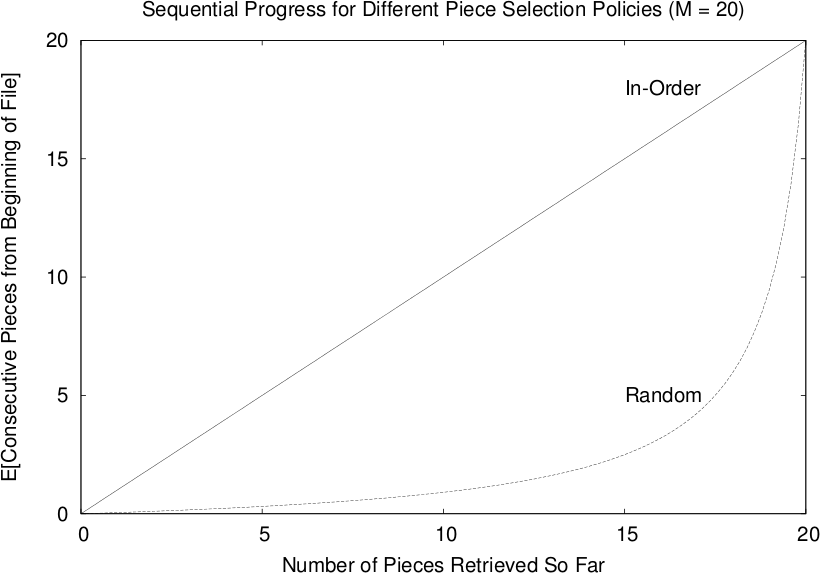
\includegraphics[width=0.5\textwidth]{src/img/multimedia-dist/sequential-progress}
  \caption{Sequential Progress}
  \label{fig:multimedia-dist:sequential-progress}
\end{figure}

As expected the \textit{random} strategy results in poor sequential progress,
albeit good download progress. Although not useful as a policy for
Peer-to-Peer streaming, this policy makes out a good point of reference, since
no other algorithm may have a poorer sequential progress. One may notice a
wide space between the \textit{random} strategy (poorest choice) and the
\textit{strictly in order} strategy (best choice). This suggest the
possibility of strategies that may be developed to still allow good
sequential progress but do not compromise the inherent behavior of the
BitTorrent protocol.

Presuming, as it usually is the case, a connection that possesses a bandwidth
capacity higher than the playback rate, an efficient streaming doesn't need to
employ \textit{strictly in order} piece selection. It only needs a sufficient
number of packages that allow content playback to happen at a consistent rate,
while other pieces may be retrieved using other algorithms. A compromise needs
to be negotiated between sequential progress and download speed, download
latency and swarm health.

In order to achieve that compromise, we define \textit{deadline pieces}. This
pieces use a deadline specifying when the packet needs to be downloaded. Such
a packet receives a priority in the pieces selection if it's close to its
deadline. This way, some of the packets may be downloaded through
\textit{rarest-first} while others may be downloaded through \textit{strictly
in order}. Deadlines may be computed by taking into account the media bitrate
and the number of pieces of the video asset.

\subsection{Design and Implementation of a Streaming Component in libtorrent}
\label{subsec:multimedia-dist:libtorrent-design}

The module implementing the piece selection is a central component in a
BitTorrent implementation. It is optimized in libtorrent to rapidly find
rarest pieces. It keeps a list of available pieces, sorted by rarity, and
equally rare packets are mixed. The \textit{rarest-first} model is the main
strategy for piece selection. Other models are supported, though their use is
particular to certain situations.

The piece selector allows combining the availability of a given packet with a
certain piece priority. These parameters determine the criterion used for
sorting the piece list. Zero priority pieces will never be selected, an option
used for selective downloading.

libtorrent-rasterbar encapsulates important components of the implementation
in several classes:
\begin{itemize}
  \item \textit{session} -- manages torrent sessions;
  \item \textit{torrent} -- defines everything regarding a torrent and its
  file;
  \item \textit{piece\_picker} -- the piece selection algorithms;
  \item \textit{peer\_connection} -- characterization of connections to
  neighboring peers.
\end{itemize}

The \texttt{piece\_picker::pick\_pieces()} function is invoked each time a
piece is selected.

For \textit{strictly in order} implementation, a specialized option dubbed
\textit{sequential} is added to the piece picker and is checked inside the
\texttt{piece\_picker::pick\_pieces()} function. A \textit{cursor} variable is
inserted that stores the index of the last downloaded piece. The interested
block list is appended the block not already download that can be downloaded
sequentially from the given peer. New blocks are added in the same manner
until the requested block limit is reached or no more pieces are available. To
be remarked that piece request is sequential but not necessarily piece
delivery.

In order to implement the \textit{piece deadline} strategy, a new concept was
added: \textit{time\_critical\_pieces}; these pieces differ from normal pieces
by having a deadline attached (\textit{piece\_deadline}). Within the library,
these pieces are requested in a different manner than normal pieces. Usually,
after a peer completes a request, a new piece request is sent to that peer.
For \textit{deadline} pieces, peer list is searched for peers possessing that
piece. Peers are sorted by download speed and outstanding bytes.

Several methods were added that allow setting up a deadline for pieces and
requesting \textit{deadline pieces}:
\textit{torrent::request\_time\_critical\_pieces()}. The peer possesses a list
of time critical pieces; the first piece is dequeued and is requested. A new
option was added to the commanding interface to allow the \textit{deadline
piece} model.

Both for the \textit{piece deadline} strategy and the \textit{strictly
in-order} strategy, there are performance gains if partially available pieces
are prioritized; that is pieces whose block are already available to the peer.
Special thanks go to Arvid Norberg, the main developer behind
libtorrent-rasterbar. He had provided useful tips, suggestions and support
both and the IRC channel and the developer's mailing list.

\subsection{Results}
\label{subsec:multimedia-dist:libtorrent-results}

In order to test the implementation, a specialized TUI interface had been
designed and implemented. This interface prints out small bars for each piece
information available. For a sequential algorithm, one can notice the ordered
piece by piece availability to a peer.

A sample graph comparing the \textit{rarest first} (blue), \textit{sequential}
(red) and \textit{deadline piece} (yellow) algorithms is shown in
Figure~\ref{fig:multimedia-dist:libtorrent-evolution}. The two
graphs show download evolution (in megabytes) and speed evolution (in KB/s).
The swarm used consisted of several seeders and a high number of leechers.
File size was 37~MB, and the file was spread into 578 pieces.

\begin{figure}
  \centering
  \subfloat[Download Size Evolution]{
  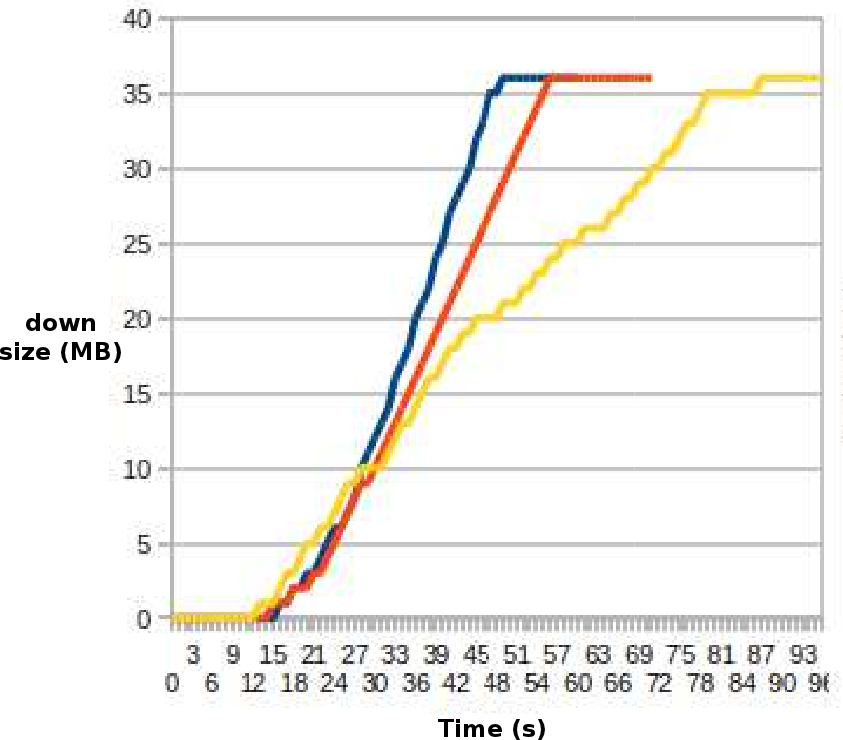
\includegraphics[width=0.48\textwidth]{src/img/multimedia-dist/libtorrent-down-size}
  \label{fig:multimedia-dist:libtorrent-down-size}
  }
  \subfloat[Download Speed Evolution]{
  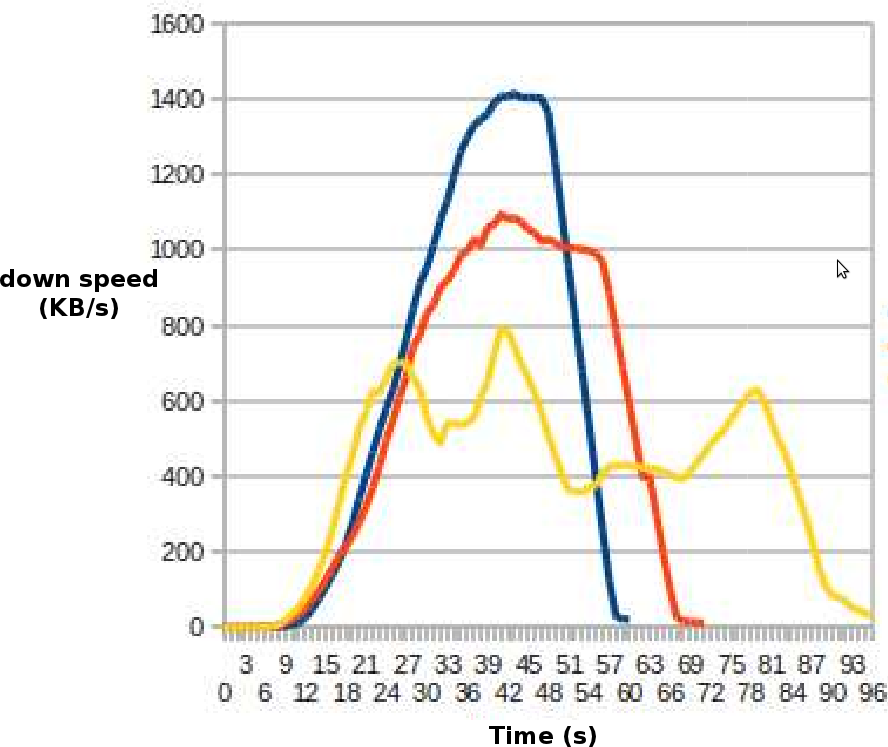
\includegraphics[width=0.48\textwidth]{src/img/multimedia-dist/libtorrent-down-speed}
  \label{fig:multimedia-dist:libtorrent-down-speed}
  }
  \caption{Evolution of Different Piece Selection Policies}
  \label{fig:multimedia-dist:libtorrent-evolution}
\end{figure}

During this experiment, the best algorithm was, as expected, the
\textit{rarest first}. We estimate the \textit{deadline piece} was
outperformed by the \textit{sequential} algorithm, due to the file size being
quite small, a large number of seeders and the implementation overhead of the
former for a relatively small file.

\section{Using Next-Share Technology for P2P Streaming}
\label{sec:multimedia-dist:nextshare}

The P2P-Next project was started in 2008 as an EU FP7 project. It aims at
delivering the next-generation Peer-to-Peer content delivery platform. The
project takes into account the change in the audio video media landscape, with
increased demand for content availability on the Internet and user participation
in generation of content. P2P-Next takes into account existing challenges such
as legal frameworks and business constraints to create a viable solution with
widespread adoption.

Intelligence, resource management, and explicit memory are the foundations for
the P2P-Next content sharing platform called: Next-Share. The Next-Share
system is a self-organizing system with complete decentralisation and hence
lacks any central bottleneck or choke points that may hamper performance,
induce setup cost, or require maintenance. Networking effects ensure that
content, communities, communication, and commerce will flourish with more
participants.

As the Next-Share technology is intrinsically intertwined with video technology,
choosing the best technology and providing efficient resource usage are part
of the goals. The technology is currently able to provide efficient access to
high definition (HD) video assets. As the codec industry is heavily
fragmented, there isn't a single solution for encoding content. As such, the
Next-Share technology relies on available implementations for content delivery
being able to render videos using such codecs as H.264, Ogg Theora, VP8.

\subsection{Next-Share Architecture and Features}
\label{subsec:multimedia-dist:nextshare-arch}

NextShare is a complex architecture integrating features that are common to
BitTorrrent applications but also those integrating streaming content. A
detailed view of the architecture is presented in
Figure~\ref{fig:multimedia-dist:nextshare-architecture}.

\begin{figure}
  \centering
  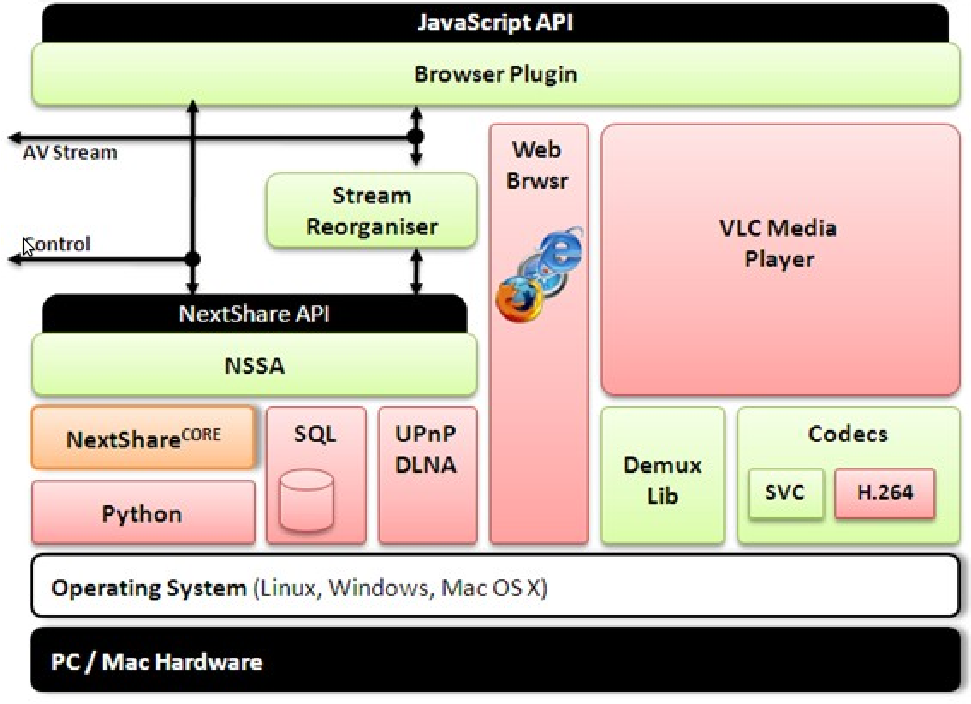
\includegraphics[width=0.7\textwidth]{src/img/multimedia-dist/nextshare-architecture}
  \caption{NextShare Architecture}
  \label{fig:multimedia-dist:nextshare-architecture}
\end{figure}

NextSharePC runs on PC, supporting Windows, Linux and MacOS X Operating
Systems/distributions. NextSharePC application is formed by two parts:
\begin{itemize}
  \item A back-end server called NextShare Agent (NSSA), which embeds the P2P
  core engine (NextShareCore).
  \item A front-end part in charge of providing the user interface and content
  playback functionalities.
\end{itemize}

The two parts typically run on the same PC and communicate through two local
socket based interfaces:
\begin{itemize}
  \item \textbf{The Control Interface}: it permits the front-end to control
  the NSSA through an API that exports NextShareCore functionalities.
  \item \textbf{The AV Streaming Interface}: the Control Interface permits to
  ask the NSSA to retrieve a media content from NextShare P2P network. The AV
  Streaming Interface is used by the NSSA to stream the retrieved content to
  the front-end. It is implemented with a local HTTP connection.
\end{itemize}

The split between front-end and back-end let the P2P engine (NSSA) run in the
background regardless if the front-end interface (GUI) is running or not. This
enables the peer to share content within the NextShare network even if the
user is not in front of the PC and/or is not interacting with NextSharePC.

The stream reorganizer is a block which permits the delivery of SVC encoded
video contents on top of codec agnostic mechanisms of NextShareCore.

For the design and the implementation of the front-end part of the platform
and in particular for the design of the GUI, the choice of the project was to
give priority to technologies coming from the web which are based on HTML5 and
JavaScript technology.

The core presents two interfaces: a GUI and a web-based plugin. The GUI is the
first version of the NextSharePC, while the web-based plugin is the second
version. In both cases the front-end is relying on VideoLan Client to
reproduce the content retrieved from NextShare network. Initial versions of
NextSharePC integrate standard releases of VLC, in future planned support of
SVC encoded video streams and adaptive play-out of media contents will require
the integration of additional plug-ins and modifications which are currently
being designed by the proof-of-concept prototyping part of the integration.

\subsubsection{Video-on-Demand in Next-Share}

Initially an improved BitTorrent core aiming for improved performance and
diverse features, the Next-Share core integrated streaming support. This has
been mostly due to Jan David Mol's
work~\cite{give-to-get}~\cite{design-p2p-live} in getting streaming
support in Next-Share. Currently, Next-Share supports both Video-on-Demand
and live streaming. Both stream features are enabled through the use of
mesh-like overlays, regarded as swarm topologies, due to their working on top
of BitTorrent.

VoD support in Next-Share is enabled through the deployment of Give-to-Get, a
novel approach to negotiating piece exchange. Give-to-Get features many
similarities to BitTorrent's own tit-for-tat protocol, but differs in certain
areas which make it more suitable for video-on-demand. Specifically, while in
offline download mode (classical distribution), the tit-for-tat protocol marks
a peer's ``altruism'' by its history, Give-to-Get only checks its recent
history. In VoD, a peer is interested in exchanging information from peers that
can offer him current pieces, in order to sustain video playback; if a peer
has been altruistic with early pieces if of little relevance to the current
peer.

As with classical BiTorrent, Give-to-Get splits the file in pieces and, based
on its neighbor set, decides which neighbor is allowed to make requests and
when requests may be unchoked. Give-to-Get implements a new unchoking
algorithm based on ranking its neighbors, based on how well a neighbor is
forwarding chunks. There are three set out of which a piece may be part of:
the high-, mid- and low-priority set as presented in
Figure~\ref{fig:multimedia-dist:gtg-sets}. \textit{h} is a parameter dictating the amount of
clustering of chunk requests in the part of the video yet to be played back.

\begin{figure}
  \centering
  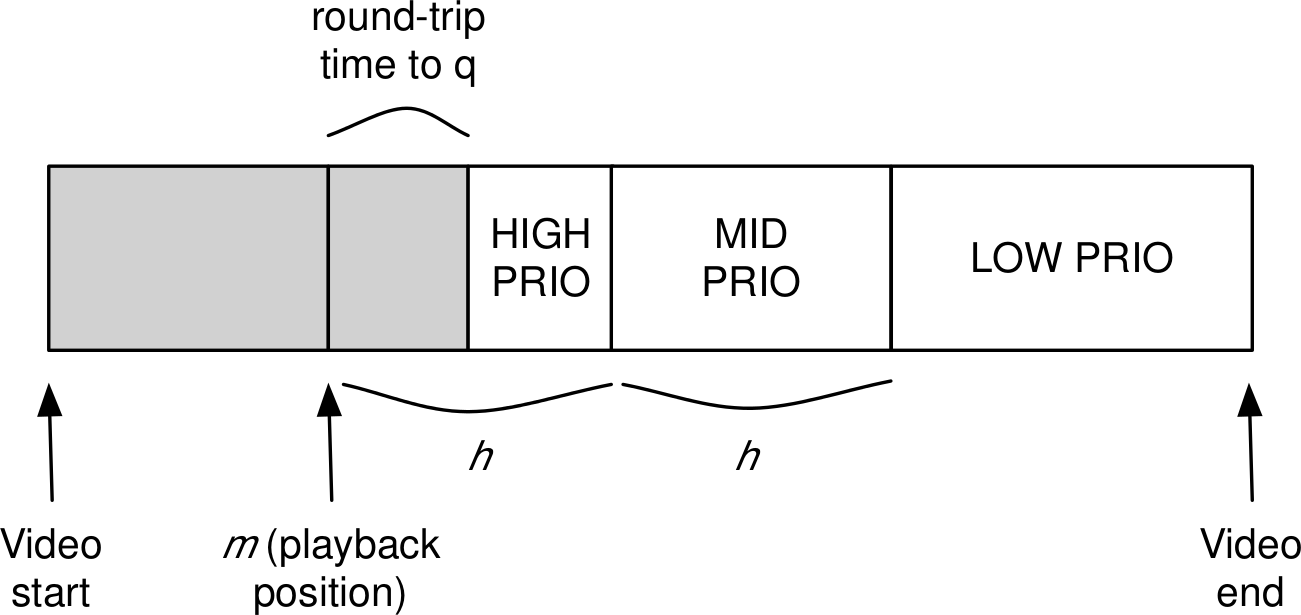
\includegraphics[width=0.5\textwidth]{src/img/multimedia-dist/gtg-sets}
  \caption{Give-to-Get Piece Sets}
  \label{fig:multimedia-dist:gtg-sets}
\end{figure}

\subsubsection{Live Streaming in Next-Share}

While most implementation use a tree-based or multi-tree based approach for
live streaming, Next-Share's BitTorrent core required a swarm-based approach.
Each peer will connect to a given set of peer and request pieces from those.
Major updates had to be undertaken due to the differences between offline
playback (classical distribution) and live streaming: the size of the file is
unknown, there is no seeder, there are no hashes for integrity checking,
pieces have to be retrieved real time. This required careful updates to the
piece picking component of the BitTorrent engine and the selection of peers in
the neighbor set.

Three types of peers are defined:
\begin{itemize}
  \item \textit{injector} -- the video source
  \item \textit{seeder} -- a peer which is always unchoked by the injector
  \item \textit{leecher} -- a peer that is not an injector or seeder
\end{itemize}

The classical definition for a seeder is no longer available as data is
generated live.

As BitTorrent is expecting the whole file to be available within a swarm,
updates have to be undertaken to ensure live streaming. The video is thus
assumed to be of ``unlimited length''. As such, the injector obtains the
video from a live source, such as a DV camera, and generates a .tstream file,
which is similar to a torrent file but cannot be used by BitTorrent clients
lacking our live streaming extensions. An end user (peer) which is interested
in watching the video stream obtains the .tstream file and joins the swarm
(the set of peers) as per the BitTorrent protocol.

A seeder is redefined in a live streaming environment to be a peer which is
always unchoked by the injector and is guaranteed enough bandwidth in order to
obtain the full video stream.The injector has a list of peer identifiers (for
example, IP addresses and port numbers) representing trusted peers which are
allowed to act as seeders if they connect to the injector. The relationship
between the injector, seeders and leechers is shown in
Figure~\ref{fig:multimedia-dist:ls-injector-seeder}. The seeders and leechers use the exact
same protocol, but the seeders (bold nodes) are guaranteed to be unchoked by
the injector (bold edges). The identity of the seeders is not known to the
other peers to prevent malicious behaviour targeted at the seeders.

\begin{figure}
  \centering
  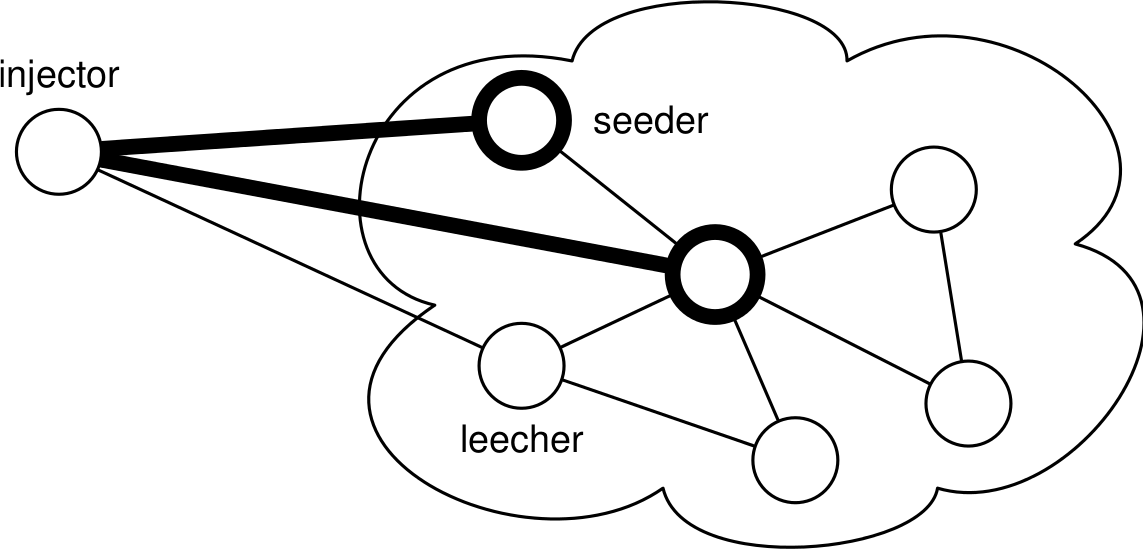
\includegraphics[width=0.5\textwidth]{src/img/multimedia-dist/ls-injector-seeder}
  \caption{Seeders in a Live Streaming Setting}
  \label{fig:multimedia-dist:ls-injector-seeder}
\end{figure}

The injector and seeders behave like a small Content Delivery Network (CDN).
Even though the seeders diminish the distributed nature of the BitTorrent
algorithm, they can be required if the peers cannot provide each other with
enough bandwidth to receive the video stream in real-time.

\subsection{NextSharePC}
\label{subsec:multimedia-dist:nextshare-pc}

NextShare is designed to run on consumer hardware most commonly found
nowadays. NextSharePC is the integrate application of the NextShare core and
PC components; it's a BitTorrent core coupled with features of NextShare and a
user interface. NextSharePC is explicitly design to attract user into the
P2P infrastructure and market the usage and advantages of the NextShare
technology.

The basic interface of the NextShare core is the Tribler
client~\cite{tribler-social}. Tribler is friendly user interface similar to
that of other BitTorrent clients. It allows complete access to the NextShare
features such as upload and downloading content, creating .torrent files and
accessing social networking features. Tribler also features a command line
interface which is useful for automatically deploying scenarios.

From a content point of view, NextShare features the SwarmPlayer interface
which is specifically direct towards video playback. The SwarmPlayer is a
simple interface that makes use of VLC technology running on top of the
NextShare core. SwarmPlayer renders video streams which are identified by a
.tstream file. It subsequently acts as a BitTorrent client sharing streaming
information.

The SwarmPlayer is an actual application running on Linux and Windows. In
order to allow easier and faster access to given content, the SwarmPlugin has
been developed. SwarmPlugin is a browser plugin that enables video playback
directly inside the browser. Currently, Firefox, IE and Safari are enabled on
Windows and Mac platforms. The SwarmPlugin is a SwarmPlayer inside a browser
making use of VLC technology. From an interface point of view is similar to
the SwarmPlayer. Actions such as fast forward, sound volume and others have to
be enabled through the use of specialized VLC JavaScript API
\footnote{\url{http://wiki.videolan.org/Documentation:WebPlugin}}.

VLC (\textit{Video LAN Client}) has been chosen due to its ubiquity and the fact that it's an open-source
project, meaning availability of the source code and a capable community. VLC
provided playback implementation for various codecs and could be easily
integrated on top of the NextShare core. The core is codec agnostic -- it
sends and receives pieces of information, leaving the decoding to an external
application, embodied as VLC. VLC support has been enabled since version
0.8.6f to version 1.1.5. VLC allowed the development of the web-based
plugin using NextShare technology -- SwarmPlugin.

With the advent of HTML5, focus has been given on running video playback
inside o browser using this technology. Currently this is enabled on Firefox,
on any platform, as it uses HTML5. While the classical VLC SwarmPlugin is
codec agnostic, HTML5-based rendering is bound to the usage of OGG Theora.

While the initial NextSharePC client, the SwarmPlayer, was designed to be a
standalone video player application, the aim for the second version was to
create a plugin for video playback in a Web browser. Allowing playback
directly in a browser makes it easier for content providers to integrate
peer-to-peer based video delivery into their existing Web based distribution
mechanisms (e.g. portals). The next version, called the SwarmPlugin consists of
plugins for the Microsoft Internet Explorer and Mozilla Firefox browsers. The
plugins support peer-to-peer based video-on-demand and live broadcasts, as
did the SwarmPlayer.

Content providers can use the plugin in their Web sites. First, they setup the
required publishing infrastructure consisting of a Next-Share tracker server
(to enable peers to find each other) and some Next-Share seeder servers (for
providing the content initially). Second, as before, they use the Next-Share
injection tools to create a .tstream metadata file for each piece of content
(containing the tracker addresses, name and bitrate of the content and
information for integrity checking the received content). Third, they upload
these .tstream files to a Web server.

The SwarmPlugin itself can be controlled from the browser using JavaScript.
This API is called the NSPlugin JavaScript API and is currently a copy of the
original VLC plugin's JavaScript API.  As such it provides
methods for controlling playback (start,pause,resume), adjusting audio
(volume) and video parameters (full screen) and receiving debug messages. In
general, the SwarmPlugin architecture is similar to that of the SwarmPlayer,
with the Graphical User Interface part of the SwarmPlayer being replaced by a
browser plugin and JavaScript controls.

\subsection{NextShareTV}
\label{subsec:multimedia-dist:nextshare-tv}

Apart from being able to run on commodity hardware through the use of the
NextSharePC implementation, the P2P-Next consortium delivers the technology
on top of consumers electronics. The device that will run the NextShare core
is a Set-top Box named NextShareTV, delivered by Pioneer Digital Design.

The scope of the NextShare TV is to develop a consumer device and user
applications to aid the discovery, enjoyment, production, and proliferation of
a broad universe of legitimate digital media. All the aforementioned digital
media shall be delivered via a next generation, open source, P2P media
delivery network called NextShare. Users of the device shall be able to engage
with a social network that shall amplify their abilities to discovery, enjoy,
enhance and share digital media. Users of the device shall be able to purchase
a broad spectrum of content from niche or local programming, through
semi-professional, to premium. The consumer device shall be able to
interoperate with other networked peripherals such as mass storage, camera,
mobile, and home PC devices residing on the premises home network.

The NextShareTV satisfies a range of commercial requirements ranging from
content distribution and streaming, to personalization and user interface.
From a content point of view, the NextShareTV offers access to Live TV streams
and to video demand assets using the Peer-to-Peer technology. Recommendation
and tagging are available and users are able to become prosumers and broadcast
their own content live via a camera connected to the box. Social networking
features are currently under work, with features such as social groupings,
chat with friends, discovering what friends are watching, doing live
recommendation to friends. Special care is given to performance, with the aim
that the prebuffering phase (the playback latency) is no more than 2 seconds.
Security and content legitimacy are also taken into account to allow
secure/certified and controlled content to be rendered on the STB; security
features may also be controlled through the presence of usernames and user
profiles.

From an architectural point of view the NextShareTV combines benefits of many
worlds: a high quality Set-top Box, a specialized Linux-based OS, provided by
ST Microelectronics, the NextShare core and libraries, drivers and modules
required for rendering, decoding and data management, and a remote management
interface. In order to allow good running time, a Python RunTime was created
-- the NextShare core uses the Python programming language.

NextShareTV devices have been deployed in various LivingLab locations within
the NextShare project for testing, evaluation and Quality of Experience.
Different types have users have accessed the devices and provided valuable
feedback and information. A remote management interface had been enabled
allowing remote control of devices and the running of various experiments. An
internal testing framework had also been developed for stress testing the
device and its applications.

\subsection{Living Lab}
\label{subsec:multimedia-dist:nextshare-ll}

The Living Lab is the mechanism by which Next-Share based application get
tested ``in the while'' i.e. with real users and real environments. In the
P2P-Next project the Living Labs are located in several partner locations such
as Lancaster (UK), Tromso (Norway), Tampere (Finland), Ljubljana (Slovenia)
and Bucharest (Romania).

Living Labs provide content to users, advice on how to install and use the
NextShare technology and support. From a user point of view, a Living Lab is
identified by a site/portal that gives access to available resources. The
Living Lab is backed by an infrastructure and framework that enable the
benefits of the technology.

The UPB Living Lab consists of several commodity hardware systems kindly
provided by the NCIT cluster. These systems store content used for the Living
Lab and the applications, scripts and services that power it. All systems are
identical both from a hardware perspective and by means of software
applications and content.

The LivingLab site, described in detail in
Section~\ref{subsec:multimedia-dist:evaluation-infrastructure} provides the
interface with the help of which users access content using NextShare
technology. It possess a large number of VoD assets from various events that
are available to be played back using the SwarmPlugin. Assets are HD content
in MP4 and OGG container format. The LivingLab describes useful information to
users and provides a forum where questions may be asked and support may be
requested.

Various experiments have taken place in the UPB Living Lab, the most recent
ones being described in Section~\ref{sec:multimedia-dist:evaluation}. As the
UPB LivingLab is focused on performance management and analysis, experiments
were keen on measuring BitTorrent swarm information and gathering relevant
information. An important set of experiments have been the ``BitTorrent
Distribution Experiments''. With the help of Ubuntu and Fedora communities,
several versions of the popular distributions had been made available through
Peer-to-Peer technology. The UPB infrastructure had been enabled and prepared
seeders to provide content in various swarms. The
site\footnote{http://p2p-next.cs.pub.ro/} had been used to present images of
BitTorrent swarm evolution, such as number of peers, number of seeders,
download speed, upload speed.

In order to collect information the chosen approach involved the gathering
client-side information collection regarding client and protocol
implementation. BitTorrent clients had been instrumented to provide verbose
information regarding BitTorrent protocol implementation. These results are
collected and subsequently processed and analysed.

The undertaken approach, while not scalable, aims to collect client-centric
data, store and analyse it in order to provide information on the impact of
network topology, protocol implementation and peer characteristics. The
infrastructure provides micro-analysis, rather than macro-analysis of a given
swarm. Focus was given to detailed peer-centric properties, rather than
less-detailed global, tracker-centric information.

Seeders had been using the NextShare technology albeit, for having to run
non-interactively, made no use of the VLC component -- the CLI of the
client had been used. Specific scripts had been used to monitor the client
activity and to restart the client in case it crashes. A typical activity of
preparing a swarm was: creating the .torrent files for the content to be made
available, distributing content to other seeders, starting the initial seeder
and using BitTorrent to distribute content to other seeders, starting the
monitoring script and making content available to user. In order to process
tracker results, a specialized script was used to do real-time parsing of
tracker log files.

The current and overall goal of the trials to be deployed and the UPB Living
Lab is comparing Peer-to-Peer streaming performance and functionalities to
classical distribution. We aim to collect relevant internal information
regarding the behavior of the technology both when used for VoD streaming and
for BitTorrent swarm download and use that information for signaling points
that should be taken into account to improve streaming performance, mostly
related to peer download speed.

\section{Evaluation of P2P Streaming Solutions}
\label{sec:multimedia-dist:evaluation}

Within the UPB Living Lab, experiments that involve users, HD content and the
NextShare streaming solutions have and are currently taking place. The goal is
to provide useful information on the functionality of the solution, the user
experience and transfer performance. As the goal of the P2P-Next project
is to built the next-generation Peer-to-Peer content delivery platform, our
aim is to provide useful information regarding key factors that influence its
attractiveness. Questions such as the ones below need to be answered: Would people use this platform instead of
YouTube? Would it outperform classical video streaming? How does it compare to
classical BitTorrent distribution performance?

The employed experiments have been lab experiments as a starting point and,
subsequently, pushed for user experience and collecting feedback. Feedback has
been used to provide information to the core team, to improve the site
providing content, to update content and to spot bugs or inconsistencies.
The Living Lab site is currently operational and is logging information from
connecting clients.

A specialized class of experiments involve gathering users for a short
period of time to simultaneously access Living Lab resources and provide
feedback. This approach results in a burst of connections and data transfer. Two such
experiments have taken place in December 2010 and April 2011, more to be
scheduled in the next months.

The UPB Living Lab is the user window to the Next-Share technology. It
provides instructions on using the technology and allows access to the content
and facilities. From a user's point of view,
the Living Lab is the site/portal/frontend allowing the playback of various video
files through the use of P2P technology. In the backend, the Living Lab is
supported by systems in the NCIT cluster that store and serve content in the
form of Video-on-Demand assets.

The components of the Living Lab and their interaction are highlighted in
Figure~\ref{fig:multimedia-dist:upb-living-lab-components}.

\begin{figure}
  \centering
  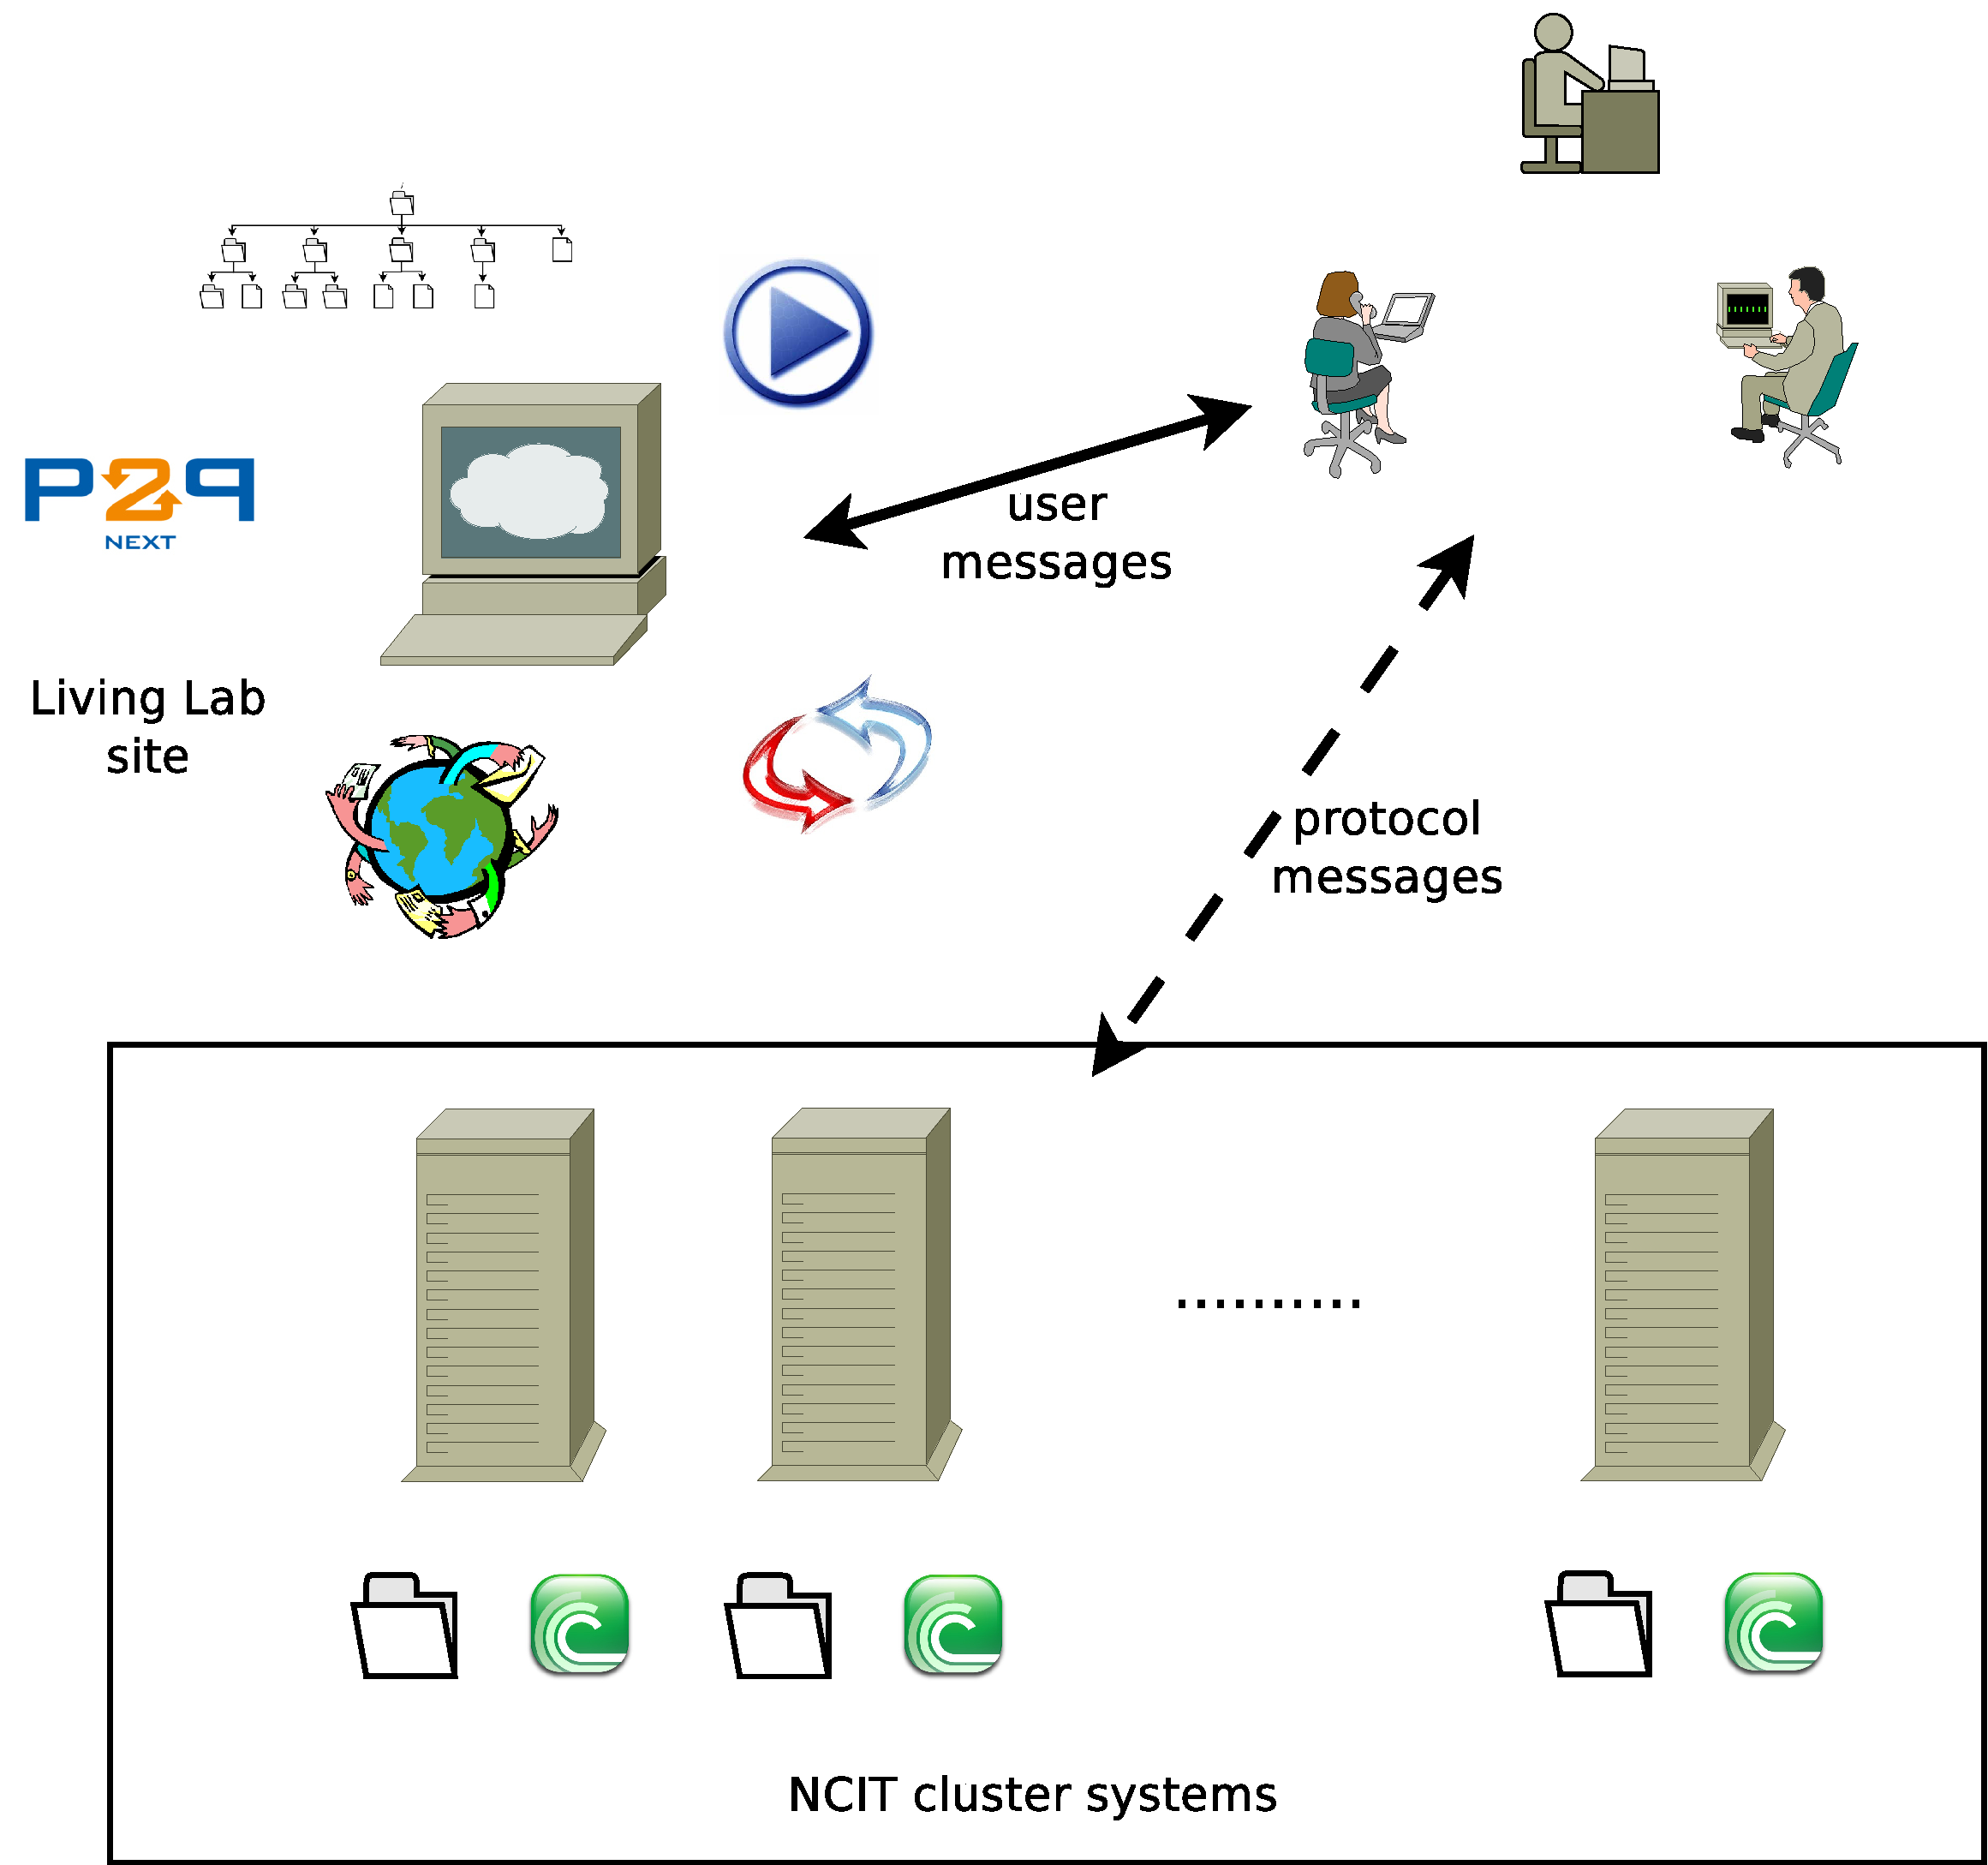
\includegraphics[width=0.7\textwidth]{src/img/multimedia-dist/upb-living-lab-components}
  \caption{Living Lab Components}
  \label{fig:multimedia-dist:upb-living-lab-components}
\end{figure}

There are three main components of the Living Lab: the NCIT cluster
systems, the Living Lab site and the users.

\subsection{Living Lab Infrastructure}
\label{subsec:multimedia-dist:evaluation-infrastructure}

The NCIT cluster systems are commodity hardware systems that provide content
and seeders. Content is replicated among NCIT cluster systems and is seeded
through automated NextShare technology applications. There are currently nine
systems available. The same content assets are found among multiple systems
such that there would be multiple seeders for each asset. Logging is enabled
at seeder level for subsequent processing. Swarm trackers may reside on a NCIT
system or outside of it; as tracker communication is reduced, its placement is
of little relevance.

The hardware systems are commodity hardware systems (2GB RAM, dual-core 3GHz
CPU, 300GB HDD) with high speed (1Gbit Ethernet) Internet links. SSH-based
access allows easy automation.

\subsubsection{Living Lab Site}

The Living Lab site~\footnote{\url{http://p2p-next.cs.pub.ro/}}), described in
Figure~\ref{fig:multimedia-dist:upb-living-lab-site}, is
the front-end users are interacting with. It provides access to NextShare
installation packages, content and support. The Living Lab site is based on
CMS Made Simple~\footnote{\url{http://www.cmsmadesimple.org/}}); it has been updated to
provide necessary features for easy content publishing, content selection and
organization. It currently provides Video-on-Demand assets (no live
streaming). Content is presented to the user in a hierarchical manner
depending on the content category. The user may access a certain
category and then select a preferred video asset.

\begin{figure}
  \centering
  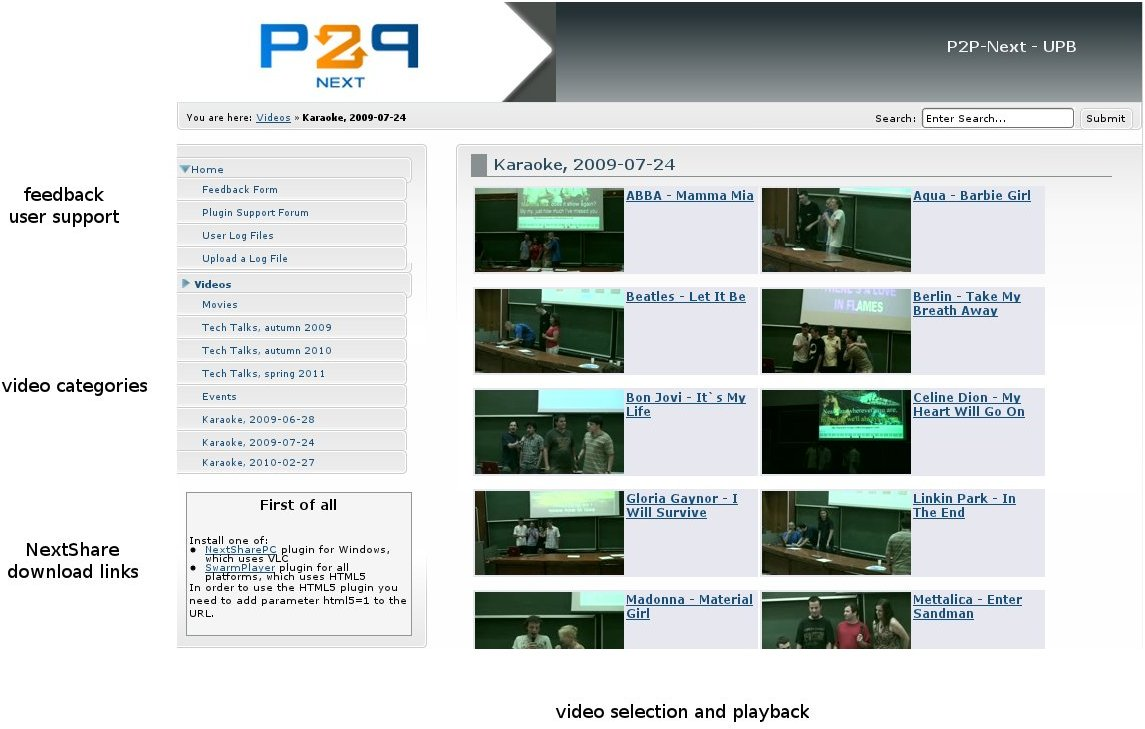
\includegraphics[width=0.5\textwidth]{src/img/multimedia-dist/upb-living-lab-site}
  \caption{Living Lab Site}
  \label{fig:multimedia-dist:upb-living-lab-site}
\end{figure}

The forum (http://p2p-next.cs.pub.ro/forum/), shown in
Figure~\ref{fig:multimedia-dist:upb-living-lab-forum} is Phorum installation (http://www.phorum.org/) allowing easy support facilities to users. The forum consists of four main categories:
\begin{itemize}
  \item Feedback and feature requests: request new features or provide
  feedback
  \item General discussions: questions regarding Living Lab Trial site and general discussions
  \item Support: request support
  \item Announcement: latest information
\end{itemize}

\begin{figure}
  \centering
  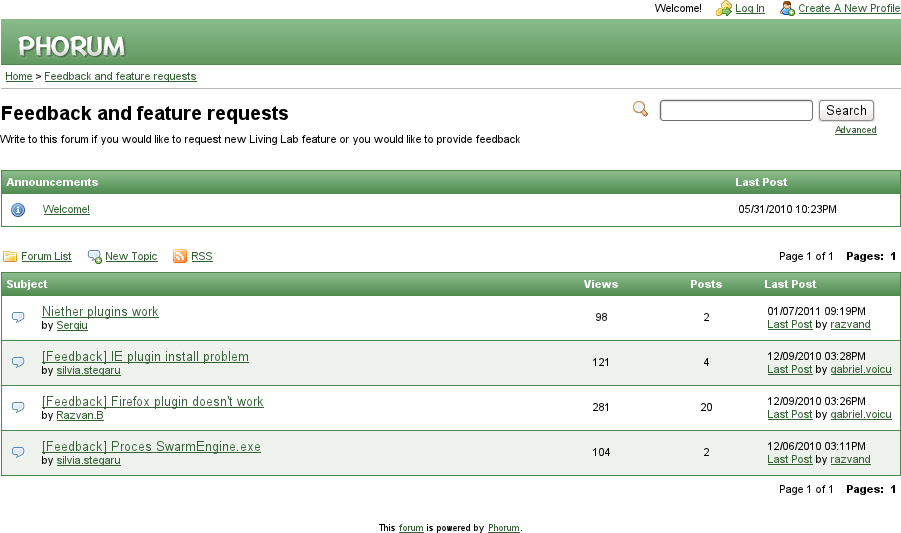
\includegraphics[width=0.7\textwidth]{src/img/multimedia-dist/upb-living-lab-forum}
  \caption{Living Lab Forum}
  \label{fig:multimedia-dist:upb-living-lab-forum}
\end{figure}

RSS feed is provided for each category, useful for notification and syncing.
There have been 29 posts and 604 views on the forum. The forum has been an
easy way for communicating with the WP4 team regarding various user reports.

User feedback is collected through feedback forms that request information
about user experience, plugins used, issues encountered. Detailed information
about feedback forms is provided in
Section~\ref{subsec:multimedia-dist:evaluation-december-2010}. The feedback
form has been updated from a Google form-based one to one that is fully
integrated into the site. At the same time, during experiment evolutions,
questions were added or were discarded. Questions that related to the user's
OS, IP address and other technical information have been discarded as they
could be deduced from connection of logging information. The current feedback
version is integrated into the site and uses a MySQL backed for storing
information. Feedback results and resulting actions are presented in
Section~\ref{subsec:multimedia-dist:evaluation-december-2010}.

A specialized form of user feedback is user log files. During experiments,
both from our side and from WP4 team members, we have requested users to
provide us with logging information for troubleshooting issues. As such, we
have integrated a log upload facility where users can upload basic upload
information provided by NextShare. Log files are typically no greater than
100K, such that there is little overhead or burden in uploading them.

Users are typically students at the Automatic Control and Computers faculty.
Various trials have asked them to participate in the trial and take part in
accessing the site, using NextShare technology for P2P streaming, giving
feedback. The Living Lab site provides links to NextShare technology
installation packages, content and other required information. Users are
contacted through e-mail and asked to participate, with links to instructions
and trial goals. Communication is thereafter handled either through e-mail or
through the forum.

A user has no information about the NCIT infrastructure system. All his/her
requests and replies are handled by the Living Lab site. However, each time
the local NextShare application is started, connection and communication are
directed towards the seeder systems. As with Peer-to-Peer technology, protocol
information is handled both through client-seeder communication and
client-client communication. The initial bootstrap phase, however, requires
communication to the seeder. Seeder logging is enabled in order to provide
information about client connections, and client-seeder communication quality.

\subsubsection{Living Lab Content}

For the LivingLab we are using videos from technical presentations, courses,
conferences and social events from our university. Most of them were shot with
a Sony Full HD camera, specified as 1080i, i.e. 1080 pixels on height,
interleaved. Although the resolution is 1440x1080, which defines an aspect
ratio of 4:3, the perceived aspect ratio is 16:9 because this is the PAR
(pixel aspect ratio). The raw movie stream loaded from the camera is packed
into a .mts multimedia container, which is based on the MPEG-2 Transport
Stream container format.

The audio stream has an AC-3 (Audio Coding 3, Dolby Digital) format, which
permits the coding of 6 surround channels. The sampling rate of 48 kHz is
higher than the CD one, which is 44.1 kHz offering a better sound fidelity.
The video stream is coded with an H.264/AVC format, a high performance video
codec defined in MPEG-4 and ITU-T standards.  The frame rate is 25 fps (frames
per second) and the overall bit rate of the raw stream is 3982 kilobits per
second, which is quite big, thus it needs compression in order to distribute
the content over the Internet. Some of the movies need to be cut into pieces
and others need to be joined together.

The number of video assets offered today is 480, occupying 61.77 GiB on our
hard-disks. The videos length ranges from a few minutes, from the social
events, about half an hour, the technical presentations, to more hours, like
the movies. The movie with the biggest length is the one which renders the
Norway tour by train which has 5 hours and 39 minutes. Occasionally we provide
live streams, but currently there is no live stream offered by UPB LivingLab.

The availability of the videos has been made possible by seeding each video in
5 five different systems. So if a system fails, enough seeders remain alive in
the swarm so that the movies are still available. This replication also
increases the speed when a movie is downloaded by a plugin. 5 of the systems
are used for seeding Ogg videos and the other 5 for MP4 videos, offering load
balancing of the hardware resources.

If a seeder client crashes a monitoring system automatically informs the
administrator of the problem so that he can restart the seeder. The tracker
and all the seeder clients provide logging. The IP of any user can be obtained
with additional statistics of its download speed evolution and clients
connected so that this information ca be afterwards joined with the feedback
provided by that user.

On the LivingLab the videos are grouped in four major categories:
\begin{itemize}
  \item Movies
  \item Technical Talks
  \item Events
  \item Karaoke
\end{itemize}

\subsection{Goals}
\label{subsec:multimedia-dist:evaluation-goals}

The current and overall goal of the trials to be deployed and the Living
Lab is comparing Peer-to-Peer streaming performance and functionalities to
classical distribution. We aim to collect relevant internal information
regarding the behavior of the technology both when used for VoD streaming and
for BitTorrent swarm download and use that information for signaling points
that should be taken into account to improve streaming performance, mostly
related to peer download speed.

We aim to use status information such as peer download speed, peer upload
speed, number of connections and extensive information (usually provided
through verbose logging) such as protocol messages, protocol inner workings,
piece picker algorithm (piece selection) to compare and analyze classical
(pure BitTorrent-based data distribution) to video streaming (through
NextShare technology). We aim to distinguish among the various patterns
employed by each type of distribution, measuring variation/penalty in
performance and identify weak and strong spots in each of the approaches.

A basic form of data collection would be from the swarm tracker. Though
information is pretty scarce (only available with each announce message
provided by the peer) it will still provide an overall view of swarms, number
of peers and their dynamics. We have been successfully using a tracker
monitoring service for classical distribution experiments and we plan to
integrate it in the near future experiments.

An important place for information storage it the Living Lab statistics
facility currently hosted at ULANC. As mentioned in Section 5, we would like
to know whether it is still operational and whether it has been restarted and
old information purged.

The main provider of status and extensive information are the peers
themselves. Each peer uses log files to store information regarding its
behavior and download sessions. As extensive logging results in high volume
information, this may only be enabled on peers we have control over, such as
seeders residing the NCIT cluster infrastructure. Verbose logging has to be
enabled in a modified version of the NextShare plugin in order to allow
retrieval of extensive information.

Status information may be provided through uploading local log files or
through the Living Lab statistics facility. Extensive logging information may
still be collected from the local seeders residing on the NCIT cluster
infrastructure. This will provide valuable information for subsequent
analysis.

As comparison between classical distribution and video delivery should
consider the same context, we aim to persuade our users to also use a
classical distribution client (maybe a non-streaming version of NextShare)
within a session. The two sets of data will form the basis for comparison
dissemination. We still have to investigate whether this is achievable and
easy would it be on the seeders side (where verbose logging is enabled) to
differentiate between the two kinds of sessions.

\subsection{Experiments}
\label{subsec:multimedia-dist:evaluation-december-2010}

During December we have undertaken a
medium-sized experiment for evaluating the NextShare technology and user
satisfaction. The Living Lab site was the center of the experiment: it
provided the interface for download the NextShare plugin, linking video files,
publishing the feedback form and providing support through the forum.

Version 1.1.0 of the NextShare plugin/SwarmPlugin (stable as of August 2010)
had been deployed for this trial. It allows the use of VLC-based NextShare
technology as a browser plugin on Windows platforms using Internet Explorer or
Mozilla Firefox. The lack of availability of the plugin for the Linux platform
had been a complaint on the feedback form, as user were part of the technical
"geek crowd".

The trial goals revolve around the generic objective of providing feedback and
bug reports to WP4 and related packages, measure user satisfaction and promote
NextShare technology and the particular objective and comparing classical
P2P/BitTorrent distribution against P2P-based video streaming, such as
provided by NextShare.

The video files deployed are those presented HD content, 3 to 30 minutes
length videos, Video-on-Demand. Most content had been converted from AVCHD
content to AVI container using H.264. The choice of AVI container did pose
some problems, and had been removed for
subsequent trials. All video files had been replicated on all available NCIT
cluster systems. Each system had started a seeder for all video asset. As
such, for each video asset there would be a number of seeders equal to the
number of cluster systems, allowing a potential overall bandwidth of 9 x 1Gbit
= 9Gbit.

Users were mostly students at the University POLITEHNICA of Bucharest. They
were contacted through email and support and communication had been ensured
through the use of the forum or private e-mail messages.

The feedback form, accessible from the Living Lab site, consisted of usability
inquiries, technical aspects and general user satisfaction. Feedback questions
were the ones described below:
\begin{itemize}
  \item Did you have any problems during the installation?
  \item Did you successfully install the SwarmPlugin?
  \item How would you classify the quality of the video playback?
  \item How would you classify the plugin's interface?
  \item What OS are you running?
  \item What browser did you use for testing the SwarmPlugin?
  \item What are your computer hardware specifications?
  \item Do you have any comments, remarks or suggestions?
  \item What was the average download speed?
  \item What version of the browser are you running?
  \item What is your external IP network address?
  \item What videos did you watch?
  \item In case of problems, what were the issues you encountered?
\end{itemize}

After the trial and discussions within the WP8 team, some of the questions had
been eliminated as information regarding the operating system or browser
version could be determined from peer connection to the seeders. The feedback
form had been implemented as a Google spreadsheet/form.

A total number of 55 users completed the feedback form. A brief of the
results:
\begin{itemize}
  \item 13 users had problems installing the plugin and most of them were
  unable to properly start the playback;
  \item video playback was deemed mediocre (a score of 2.4 out of 5); some may
  be due to the problems in installing the plugin;
  \item the plugin interface was considered to be usable - content playback
  could be easily enabled;
  \item most users used the Firefox version of the Plugin;
  \item users were using high bandwidth connections ($>$ 512KB/s) or fairly
  good ones ($>$ 50KB/s, $<$ 100KB/s);
  \item video freezing and the lack of a seek and volume bar were among the
  most significant remarks.
\end{itemize}

In order to collect information regarding the problems, FTP-based upload form
to allow users to provide us their log files.

The most important issues were problems during the installation and poor video
playback (freezing). One of the main results A similar experiment would need
to provide proper video content (if the problem is from video files), a
properly working version of the NextShare plugin and a seek bar on the
playback interface.

The forum was heavily utilized during this period, as users experienced
various problems with installing the plugin and making it work both on
Internet Explorer and on Firefox. There have been 29 posts and 604 views on
the forum. The forum has been an easy way for communicating with the WP4 team
regarding various user reports. A total of 17 users created and used accounts
on the forum.

\subsection{Issues and Feedback}
\label{subsec:multimedia-dist:evaluation-issues}

\subsubsection{Results of Experiments}

42 users had correctly presented their IP addresses. We have used the
excellent IPInfoDB location API (http://www.ipinfodb.com/ip_location_api.php)
to determine their geolocation:
\begin{itemize}
  \item 37 users from Romania
  \item 3 users from the Netherlands
  \item 1 user from France
  \item 1 user from UK
\end{itemize}

The feedback form had provided results as shown in
Table~\ref{tab:multimedia-dist:december-2010-results}.

\begin{table}[htb]
  \centering
  \caption{December 2010 Trial Feedback Report}
  \label{tab:multimedia-dist:december-2010-results}
  \begin{tabular}{@{}ll@{}}
    \toprule
      \textbf{Feedback question} & \textbf{Feedback response} \\
    \midrule
      \multirow{2}{*}{Did you have any problems during the installation?} &
      Yes: 13 \\
       & No: 42 \\
    \midrule
      \multirow{2}{*}{Did you successfully install the SwarmPlugin?} & Yes: 52
      \\
       & No: 3 \\
    \midrule
      How would you classify the quality of the video playback? & Average:
      2.41 (out of 5) \\
    \midrule
      How would you classify the plugin's interface? & Average: 3.02 (out of
      5) \\
    \midrule
      \multirow{5}{*}{What OS are you running?} & Win XP: 12 \\
       & Win Vista: 10 \\
       & Win 7: 23 \\
       & Win 7 (64bit): 8 \\
       & Win Server 2008: 2 \\
    \midrule
      \multirow{3}{*}{What browser did you use for testing the SwarmPlugin?} &
      Internet Explorer: 10 \\
       & Mozilla Firefox: 28 \\
       & Dual (IE \& FX): 17 \\
    \midrule
      \multirow{5}{*}{What was the average download speed?} & less than
      50KB/s: 14 \\
       & between 50KB/s and 100KB/s: 6 \\
       & between 100KB/s and 256KB/s: 7 \\
       & between 256KB/s and 512KB/s: 3 \\
       & above 512KB/s: 25 \\
    \bottomrule
  \end{tabular}
\end{table}

Users had found the plugin and technology fun to use and provide feedback,
both from an average user's perspective and from a technical user's
perspective. Features that have been praised were:
\begin{itemize}
  \item Fast download speed.
  \item Easy installation.
  \item Good video quality.
\end{itemize}

Users reported a variety of issues, most of which have been tackled for the
Living Lab site or asked fro support from the NextShare core (WP4) team.
Requests, suggestions and issues were:
\begin{itemize}
  \item The lack of a plugin for Google Chrome.
  \item The lack of a plugin for the Linux platform.
  \item The inability to choose an installation directory or a caching
  directory. Resulted in no more space being available.
  \item Playback is "freezing" or choppy "freezing".
  \item The lack of a volume or time/progress bar.
  \item The lack of a full screen button.
  \item High CPU consumption (as signaled in Task Manager). Many page faults
  were observed through Task Manager for the plugin process.
  \item Content diversity should be improved.
  \item Long buffering time.
  \item Difficult playback from Edinburgh, UK.
  \item Lack of reload button.
  \item Placing lower resolutions videos for playback problems and for lower
  download speed.
  \item The installer should signal what applications need to be closed in
  order to enable the plugin.
  \item Sound was missing.
  \item The installer should detect a previous version installation and point
  the user to uninstalling that first.
\end{itemize}

The issues marked in bold were signaled often. The lack of a volume or
time/progress bar was present in almost all suggestions in the feedback form.

Technical issues had also been signaled on the forum and were asked for help
from the WP4 core team. These included:
\begin{itemize}
  \item The lack of generation of a log file for troubleshooting.
  \item Incorrect permissions (on Windows 7) that prevent users from
  installing the applications. Have to enable Administrative access rights.
  \item The lack of "dual" functionality for both Internet Explorer and
  Firefox. When the plugin is installed for one of the browsers it doesn't
  work on the other.
\end{itemize}

The important issues had been tackled after the trial, some of them being
described in detail in Section~\ref{subsec:multimedia-dist:evaluation-issues}. The most stringent issue deals with
playback problems in the NextShare player for a diversity of video files. This
was due to multiple reasons. One of them of the absence of a bitrate
information in the .torrent/.tstream file; the client was unable to properly
render the video. Another cause was the 

Due to our discovery of problems regarding bitrate variation influencing
quality (or functionality) of video playback, we were considering the
possibility of providing the end user with multiple versions of the same video
file: different resolution, different bitrate, different codec, different
container. That would imply some disparate statistics but may provide the user
with better quality of experience when using a "less demanding" video file.
More on this is discussed in Section~\ref{subsec:multimedia-dist:evaluation-issues}.

The lack of a Linux plugin has been addressed by integrating the HTML5-based
plugin. The April 2011 trial had included
dual video formats that are playable through the use of the classic VLC-based
plugin and the HTML5-based plugin.

Interface requests, the most demanding of the user's replies, had been
addresses through the use of VLC Javascript API. This enabled the addition of
a progress bar, volume bar, time information, full screen button. More
information is presented in Section~\ref{subsec:multimedia-dist:evaluation-issues}.

\subsubsection{Updates as Feedback from Results}

The VLC based plugin does not provide any user interface. It only displays a
rectangle where the video is rendered. Several P2P-Next's trial sites extend
the plugin's interface by putting Play, Pause and Stop buttons. UPB LivingLab
used to have the same interface for NextSharePC, but the users where
complaining about these interface in their's feedback, demanding several
facilities.

Based on their's feedback we extended NextSharePC plugin with a JavaScript
interface which uses jQuery. The new interface includes:
\begin{enumerate}
  \item a progress bar, which shows the current position in the video and can
  be used to seek to a different position
  \item the current time of the video in minutes and second (MM:SS format) and
  also the total time (in the same format)
  \item a Fullscreen button
  \item the old Play, Pause and Stop buttons.
\end{enumerate}

All the videos have been converted in two qualities: 
\begin{itemize}
  \item SD (Standard Definition) which has a resolution of 800x600 and a
  bitrate of 700 kb/s
  \item HD (High Definition) with a 960x720 resolution and a 1400 kb/s bitrate
\end{itemize}

Each video in each quality also needed to be converted using two different
containers. The SwarmPlugin which uses HTML5 requires an Ogg container with
Theora video codec and Vorbis audio codec for compatibility with all browsers
that support HTML5 (Mozilla Firefox and Internet Explorer). For the
NextSharePC plugin which is based on VLC almost any common container and codec
can be used. That is why we chose an H.264/AVC video codec that can provide
high quality and still low bitrates and an MP3 audio codec packed in an MP4
container. Thus each video required encoding into four different versions.

The decision of using the four versions for each video described above, has
been made by experimenting with a lot of other versions by choosing different:
\begin{itemize}
  \item containers: AVI, MP4, Ogg, WebM
  \item video codecs: H.264/AVC, Theora, VP8
  \item audio codecs: MP3, AAC, Vorbis
  \item resolutions: 800x600, 960x720, 1440x1080
  \item bit rates: 525 kb/s, 700 kb/s, 875 kb/s, 1050 kb/s, 1400 kb/s
  \item frames rates (fps): 25 fps, 30 fps, 50 fps.
\end{itemize}

\section{Conclusion}
\label{subsec:multimedia-dist:conclusion}

As a large part of content is currently video, Peer-to-Peer systems have
sought out solutions for integrating streaming support. In this chapter, a
proof of concept of integrating streaming algorithms into BitTorrent
applications was the development of extra features for the popular
libtorrent-rasterbar. We have added two streaming algorithms that altered the
classical rarest piece first policy and instead focused on delivering
sequential pieces of content.

An important solution for streaming is developed by the P2P-Next
consortium\footnote{http://www.p2p-next.org/} in the form of the NextShare
technology. The NextShare technology provides extensive features for
delivering the next generation P2P media distribution framework. It provides
support for VoD, live streaming, supports VLC and HTML5 based browser plugins,
runs on PCs and STBs and is constantly evaluated within the consortium
LivingLab. The NextShare technology uses Give-to-Get~\cite{give-to-get}, an
update to BitTorrent's policy, with good performance for VoD. For live
streaming, NextShare creates mesh-based (swarm-based) overlays where several
nodes are dubbed ``seeders'' and are always unchoked by the source
node~\cite{design-p2p-live}.

The NextShare technology and its features are constantly evaluated in the
P2P-Next consortium LivingLabs\footnote{http://livinglab.eu/}. One such
LivingLab, located in UPB, provides more than 60 GB of VoD assets that may be
accessed by users through the technology in the form of browser plugin
playback.  Feedback is provided back to the NextShare core or to the LivingLab
as a whole in order to improve attractiveness and quality of experience.
Feedback is collected from users, in form of questions in feedback forms, or
from log files and messages~\cite{bt-swarm-analysis}.

The overall aim of the LivingLab is to evaluate the possibility for the
NextShare platform to be deployed and used in real environments. As a
Peer-to-Peer solution, both technical and legal challenges have to be
undertaken and LivingLabs provide the framework in which real experiments
take place.

The LivingLab in UPB relies on students, technical people and open-source
enthusiasts to participate in various surveys and provide feedback around the
technology. We are particularly interested in performance related aspects of
the platform, using measures such as peer download speed, peer upload speed,
swarm speed. The current goal is to provide an in-depth comparison of
classical distribution through BitTorrent and streaming using the updated
BitTorrent core in NextShare. We hope to provide valuable insight regarding
the behavior of the updated core and advice on improving performance and,
thus, quality of experience for users.
